% !TEX program = lualatex
% !TEX bibtex   = bibtex
% A Comparative Study of Deep RL Algorithms: DQN, PPO, SAC, TD3
% EE-568 Reinforcement Learning, EPFL, Spring 2026
% Kevin Abou Jaoude, Youssef Dib, Fuad Khuri

\documentclass[final]{beamer}

\usepackage{lmodern}
\usepackage[orientation=portrait,size=a1,scale=1.0]{beamerposter}
\usetheme{gemini}
\usecolortheme{nott}

\usepackage{graphicx}
\usepackage{anyfontsize}
\usepackage{amssymb}
\usepackage{pifont}
\usepackage{booktabs}
\usepackage{array}
\usepackage{adjustbox}
\usepackage{tikz}
\usetikzlibrary{shapes.geometric, arrows.meta, calc, decorations.pathmorphing, backgrounds, positioning, shadows, shadows.blur, fit, shapes.misc}
\input{packages}
\input{macros}
\DeclareMathOperator*{\argmax}{arg\,max}
\DeclareMathOperator*{\argmin}{arg\,min}
\usepackage{xcolor}
\usepackage{etoolbox}
\usepackage{multicol}

\newlength{\sepwidth}
\newlength{\colwidth}
\setlength{\sepwidth}{0.022\paperwidth}
\setlength{\colwidth}{0.467\paperwidth}
\newcommand{\separatorcolumn}{\begin{column}{\sepwidth}\end{column}}

\setlength{\jot}{4pt}

% Tighten vertical gap between blocks (Gemini default is too generous for a full left column)
\addtobeamertemplate{block begin}{}{\vspace{-0.3em}}
\addtobeamertemplate{block end}{\vspace{-0.4em}}{}
\addtobeamertemplate{alertblock begin}{}{\vspace{-0.3em}}
\addtobeamertemplate{alertblock end}{\vspace{-0.4em}}{}

% ---- Override the Gemini headline title to a smaller size so the title
%      fits on 1--2 lines and the EPFL logo can be smaller.
\setbeamerfont{headline title}{size=\huge,series=\bfseries}
\setbeamerfont{headline author}{size=\Large}
\setbeamerfont{headline institute}{size=\normalsize}

% ====================
% Color palette
% ====================
\definecolor{epflred}{RGB}{200,16,46}
\definecolor{softgrey}{RGB}{96,96,96}
\definecolor{cartcol}{RGB}{120,160,210}
\definecolor{pendcol}{RGB}{220,120,90}
\definecolor{mccgrass}{RGB}{120,170,120}

% Algorithm identity colors (matching matplotlib tab10)
\definecolor{dqncol}{RGB}{31,119,180}    % blue
\definecolor{ppocol}{RGB}{255,127,14}    % orange
\definecolor{saccol}{RGB}{44,160,44}     % green
\definecolor{td3col}{RGB}{148,103,189}   % purple

\newcommand{\hl}[1]{\textcolor{epflred}{\textbf{#1}}}
\newcommand{\algotag}[2][epflred]{\textcolor{#1}{\textbf{#2}}}

% ====================
% Algorithm card
% ====================
\newcommand{\algocard}[3]{%
  \begin{minipage}[t]{0.49\colwidth}
    \begin{tikzpicture}[baseline=(card.north)]
      \node[anchor=north west, inner sep=0.4em, minimum width=0.49\colwidth,
            text width=0.47\colwidth, draw=#1, line width=2pt,
            rounded corners=0.2em, fill=#1!5] (card) {%
        \begin{minipage}{0.44\colwidth}
          \textcolor{#1}{\textbf{\large #2}}\\[0.2em]
          #3
        \end{minipage}};
    \end{tikzpicture}%
  \end{minipage}%
}

% ====================
% Key-number badge
% ====================
\newcommand{\keynum}[3]{%
  \begin{tikzpicture}
    \node[circle, draw=#1, fill=#1!10, line width=2pt,
          minimum size=3.4cm, align=center, font=\bfseries] (n) {%
        \textcolor{#1}{\fontsize{26}{30}\selectfont #2}};
    \node[below=0.15cm of n, align=center, text width=4.6cm,
          font=\small] {#3};
  \end{tikzpicture}}

% ====================
% Environment cartoons (TikZ)
% ====================

\newcommand{\cartpoleTikZ}{%
\begin{tikzpicture}[scale=0.95, every node/.style={font=\scriptsize}]
  \draw[thick] (-1.2,0) -- (1.2,0);
  \foreach \x in {-1.1,-0.85,...,1.15} \draw (\x,0) -- (\x-0.08,-0.12);
  \draw[thick, fill=cartcol!50, rounded corners=2pt] (-0.55,0.05) rectangle (0.55,0.55);
  \draw[fill=black] (-0.35,0.05) circle (0.10);
  \draw[fill=black] (0.35,0.05) circle (0.10);
  \draw[fill=cartcol!90, rounded corners=2pt] (-0.45,0.55) rectangle (0.45,0.6);
  \draw[thick, line width=3pt, epflred!80] (0,0.6) -- (0.55,1.85);
  \draw[fill=epflred, draw=epflred!70, line width=1pt] (0.55,1.85) circle (0.13);
  \draw[->, very thick, epflred] (-0.75,0.30) -- (-1.15,0.30);
  \draw[->, very thick, epflred] (0.75,0.30) -- (1.15,0.30);
  \node[epflred, anchor=south] at (0,1.95) {\textbf{balance}};
\end{tikzpicture}}

\newcommand{\acrobotTikZ}{%
\begin{tikzpicture}[scale=0.95, every node/.style={font=\scriptsize}]
  \draw[thick] (-1.0,1.85) -- (1.0,1.85);
  \foreach \x in {-0.9,-0.5,-0.1,0.3,0.7} \draw (\x,1.85) -- (\x-0.12,2.05);
  \draw[fill=black] (0,1.85) circle (0.08);
  \draw[thick, line width=3pt] (0,1.85) -- (0.55,1.05);
  \draw[fill=epflred, draw=epflred!70, line width=1pt] (0.55,1.05) circle (0.09);
  \draw[thick, line width=3pt] (0.55,1.05) -- (0.15,0.20);
  \draw[fill=epflred, draw=epflred!70, line width=1pt] (0.15,0.20) circle (0.13);
  \draw[dashed, epflred, thick] (-1.05,0.50) -- (1.05,0.50);
  \node[epflred, anchor=east, font=\scriptsize\bfseries] at (1.05,0.65) {goal h};
  \draw[->, thick, epflred, dashed] (0.7,0.4) to[bend left=25] (0.3,1.4);
\end{tikzpicture}}

\newcommand{\pendulumTikZ}{%
\begin{tikzpicture}[scale=0.95, every node/.style={font=\scriptsize}]
  \draw[thick] (-0.5,1.75) -- (0.5,1.75);
  \foreach \x in {-0.4,-0.1,0.2,0.5} \draw (\x,1.75) -- (\x-0.08,1.92);
  \draw[fill=black] (0,1.75) circle (0.08);
  \draw[thick, line width=3pt] (0,1.75) -- (0.70,0.65);
  \draw[fill=pendcol, draw=pendcol!70, line width=1pt] (0.70,0.65) circle (0.22);
  \draw[->, very thick, epflred] (-0.45,1.30) arc[start angle=170, end angle=80, radius=0.65];
  \node[epflred, anchor=south west, font=\scriptsize\bfseries] at (0.1,1.95) {torque $\tau$};
\end{tikzpicture}}

\newcommand{\mccTikZ}{%
\begin{tikzpicture}[scale=0.95, every node/.style={font=\scriptsize}]
  \draw[thick, fill=mccgrass!30] plot[smooth, samples=60, domain=-1.20:1.20]
       ({\x},{0.55*\x*\x + 0.05}) -- (1.20,-0.05) -- (-1.20,-0.05) -- cycle;
  \foreach \x in {-1.1,-0.8,...,1.1} {%
    \pgfmathsetmacro{\yy}{0.55*\x*\x + 0.05}
    \draw[mccgrass!70, thick] (\x,\yy) -- (\x,\yy+0.07);}
  \draw[thick, fill=cartcol!60, rounded corners=2pt] (-0.30,0.10) rectangle (0.15,0.40);
  \draw[fill=black] (-0.22,0.10) circle (0.07);
  \draw[fill=black] (0.08,0.10) circle (0.07);
  \draw[thick] (1.05,0.65) -- (1.05,1.25);
  \fill[epflred] (1.05,1.25) -- (1.05,0.95) -- (0.72,1.10) -- cycle;
  \node[epflred, anchor=west, font=\small\bfseries] at (0.30,1.40) {+100};
  \draw[->, very thick, epflred, dashed] (-0.05,0.45) to[bend left=20] (0.95,1.15);
\end{tikzpicture}}

% ====================
% Decision tree for "When to use which algorithm"
% ====================
\newcommand{\decisionTree}{%
\begin{tikzpicture}[
    every node/.style={font=\footnotesize, align=center},
    decision/.style={diamond, draw=epflred, fill=epflred!10, line width=1.2pt, minimum width=4.8cm, aspect=2.5, inner sep=1pt},
    algo/.style={rectangle, rounded corners=0.3em, draw, line width=1.2pt, minimum width=3.0cm, minimum height=1.0cm, inner sep=3pt, font=\bfseries\normalsize},
    arrow/.style={->, line width=1.3pt, epflred},
    edgelabel/.style={font=\footnotesize\bfseries, midway, fill=white, inner sep=1pt}
]
% Top question
\node[decision] (q1) at (0,0) {Action space?};

% Discrete branch: DQN + PPO
\node[algo, fill=dqncol!15, draw=dqncol, text=dqncol, anchor=north]
   (dqn) at (-5.5,-2.6) {DQN};
\node[algo, fill=ppocol!15, draw=ppocol, text=ppocol, anchor=north]
   (ppod) at (-2.5,-2.6) {PPO};

% Right-side question for continuous
\node[decision, anchor=north] (q2) at (3.8,-2.6) {Reward sparse?};

\draw[arrow] (q1) -- node[edgelabel, sloped] {discrete} (dqn.north);
\draw[arrow] (q1) -- node[edgelabel, sloped] {discrete} (ppod.north);
\draw[arrow] (q1) -- node[edgelabel, sloped, above] {continuous} (q2.north);

% Continuous + dense -> SAC, TD3
\node[algo, fill=saccol!15, draw=saccol, text=saccol, anchor=north]
   (sac) at (1.8,-5.5) {SAC};
\node[algo, fill=td3col!15, draw=td3col, text=td3col, anchor=north]
   (td3) at (4.8,-5.5) {TD3};
% Continuous + sparse -> PPO
\node[algo, fill=ppocol!15, draw=ppocol, text=ppocol, anchor=north]
   (ppos) at (7.8,-5.5) {PPO};

\draw[arrow] (q2) -- node[edgelabel, sloped] {no (dense)} (sac.north);
\draw[arrow] (q2) -- node[edgelabel, sloped] {no (dense)} (td3.north);
\draw[arrow] (q2) -- node[edgelabel, sloped, above] {yes} (ppos.north);
\end{tikzpicture}}

% ====================
% Title block
% ====================

\title{A Comparative Study of Deep RL Algorithms: DQN, PPO, SAC, TD3}

\author[K. Abou Jaoude, Y. Dib, F. Khuri]{{\Large\textsc{\textbf{$\sim$ Team KFY $\sim$}}}\\[0.4ex] Kevin Abou Jaoude \quad Youssef Dib \quad Fuad Khuri}

\institute[EPFL EE-568, Spring 2026]{EE-568 Reinforcement Learning \, $\cdot$ \, EPFL \, $\cdot$ \, Spring 2026}

\logoright{
\includegraphics[height=4.2cm]{logos/epfl.png}}

\footercontent{
  EE-568 Reinforcement Learning \, $\cdot$ \, Applied Project 1 \, $\cdot$ \,
  Kevin Abou Jaoude, Youssef Dib, Fuad Khuri \, $\cdot$ \, EPFL, Spring 2026
}

% ====================
% Document
% ====================

\begin{document}
\begin{frame}[t]
\begin{columns}[t]
\separatorcolumn

% ============================================================
% LEFT COLUMN
% ============================================================
\begin{column}{\colwidth}

    % ---------- Environments ----------
    \begin{block}{1. Four classic-control environments}
        \centering
        \begin{minipage}[t]{0.235\colwidth}\centering
            \cartpoleTikZ \\[0.2em]
            \textbf{\algotag[cartcol!80!black]{CartPole-v1}} \\
            \small Discrete(2) \, $\cdot$ \, dense $+1$/step \\
            100k env steps
        \end{minipage}\hfill
        \begin{minipage}[t]{0.235\colwidth}\centering
            \acrobotTikZ \\[0.2em]
            \textbf{\algotag[cartcol!80!black]{Acrobot-v1}} \\
            \small Discrete(3) \, $\cdot$ \, dense $-1$/step \\
            200k env steps
        \end{minipage}\hfill
        \begin{minipage}[t]{0.235\colwidth}\centering
            \pendulumTikZ \\[0.2em]
            \textbf{\algotag[pendcol!80!black]{Pendulum-v1}} \\
            \small Box$[-2,2]$ \, $\cdot$ \, dense \\
            200k env steps
        \end{minipage}\hfill
        \begin{minipage}[t]{0.235\colwidth}\centering
            \mccTikZ \\[0.2em]
            \textbf{\algotag[mccgrass!60!black]{MCC-v0}} \\
            \small Box$[-1,1]$ \, $\cdot$ \, \hl{sparse} \\
            300k env steps
        \end{minipage}
    \end{block}

    % ---------- Setup and taxonomy ----------
    \begin{block}{2. Setup and taxonomy}
        We re-implement four canonical deep RL algorithms from scratch in PyTorch (no \texttt{stable-baselines3}) and benchmark them with 3 seeds each, 95\% bootstrap CIs over seeds, and four pre-registered ablations on four Gymnasium~[5] classic-control environments.

        \vspace{0.15em}
        \begin{center}
        \small
        \renewcommand{\arraystretch}{1.1}
        \begin{tabular}{@{}l|cc@{}}
            \toprule
                                  & \textbf{on-policy} & \textbf{off-policy} \\
            \midrule
            \textbf{value-based}  & ---            & \algotag[dqncol]{DQN} \\
            \textbf{policy-based} & \algotag[ppocol]{PPO} & \algotag[saccol]{SAC}, \algotag[td3col]{TD3} \\
            \bottomrule
        \end{tabular}
        \end{center}

        \textbf{Networks.} $(64,64)$ MLPs for DQN, PPO; $(256,256)$ for SAC, TD3 (canonical paper widths). \quad \textbf{Hardware.} RTX 3070 + EPFL gnoto V100.
    \end{block}

    % ---------- Algorithms ----------
    \begin{block}{3. Algorithms}
        \small
        \algocard{dqncol}{DQN [1]}{%
          value-based, off-policy, discrete:
          \[
          \mathcal{L} = \mathbb{E}\!\left[\ell_{\text{Hub}}\!\big(Q_\theta - r - \gamma(1{-}d)\textstyle\max_{a'}Q_{\bar{\theta}}\big)\right]
          \]
          $\varepsilon$-greedy, target sync every $\tau$ steps, Huber loss.}\hfill
        \algocard{ppocol}{PPO [2]}{%
          policy-based, on-policy:
          \[
          \mathcal{L} = -\mathbb{E}\!\left[\min\!\big(r_t\hat{A}_t,\, \mathrm{clip}(r_t, 1{\pm}\epsilon)\hat{A}_t\big)\right]
          \]
          GAE advantages, clipped surrogate as a soft trust region.}

        \vspace{0.2em}

        \algocard{saccol}{SAC [3]}{%
          off-policy, max-entropy:
          \[
          J = \mathbb{E}\!\left[\textstyle\sum_t \gamma^t\big(r_t + \alpha\,\mathcal{H}[\pi(\cdot|s_t)]\big)\right]
          \]
          Squashed-Gaussian actor, auto $\alpha$ via $\log\alpha$, twin Q.}\hfill
        \algocard{td3col}{TD3 [4]}{%
          off-policy, deterministic:
          \[
          y = r + \gamma(1{-}d)\textstyle\min_{i}Q_{\bar{\phi}_i}\!\big(s', \mathrm{clip}(\pi_{\bar{\theta}}{+}\mathrm{clip}(\tilde{\epsilon},{\pm}0.5),\,a_{\min},a_{\max})\big)
          \]
          Twin critics, target smoothing $\tilde{\sigma}{=}0.2$; \emph{two} clips required.}
    \end{block}

    % ---------- Implementation details ----------
    \begin{block}{4. Implementation details that mattered}
        \begin{itemize}
            \itemsep0.05em
            \item \algotag[dqncol]{DQN}: target-sync sweep on CartPole gives a \hl{U-shape} ($\tau\in\{100, 1000, 5000\}$). The canonical $\tau{=}1000$ sits at the edge of stability, which explains the seed-bimodality.
            \item \algotag[ppocol]{PPO}: at Pendulum truncation we fold $\gamma V(s_{t{+}1})$ into the reward so GAE accounts for the value of the truncated state; raw \texttt{done} flags bias returns by $\sim$30.
            \item \algotag[saccol]{SAC}: the tanh-Jacobian log-prob correction $-\sum_i \log(1-\tanh^2 u_i)$ is mandatory; without it the entropy term is silently wrong and training never moves off the warmup floor (verified: return stuck at $-1200$ on Pendulum without it).
            \item \algotag[td3col]{TD3}: the smoothed target action needs \emph{two} clips, on the noise ($\pm 0.5$) and on the action range. Skipping the outer clip sticks the actor on the boundary.
            \item \textbf{All four}: bootstrap mask uses \texttt{terminated} only, not \texttt{terminated\,or\,truncated}.
        \end{itemize}
    \end{block}

    % ---------- All four ablations consolidated, NOW ON LEFT ----------
    \begin{alertblock}{5. Pre-registered ablations: turning the canonical knobs}
        Four pre-registered sweeps, one per algorithm, 3 seeds each. \\
        \textbf{Headline (MCC, sparse reward):} \hl{turning the off-policy exploration knobs (SAC $\alpha$, TD3 $\sigma$) does not rescue them.}

        \vspace{0.2em}
        \begin{minipage}[t]{0.46\colwidth}
            \centering
            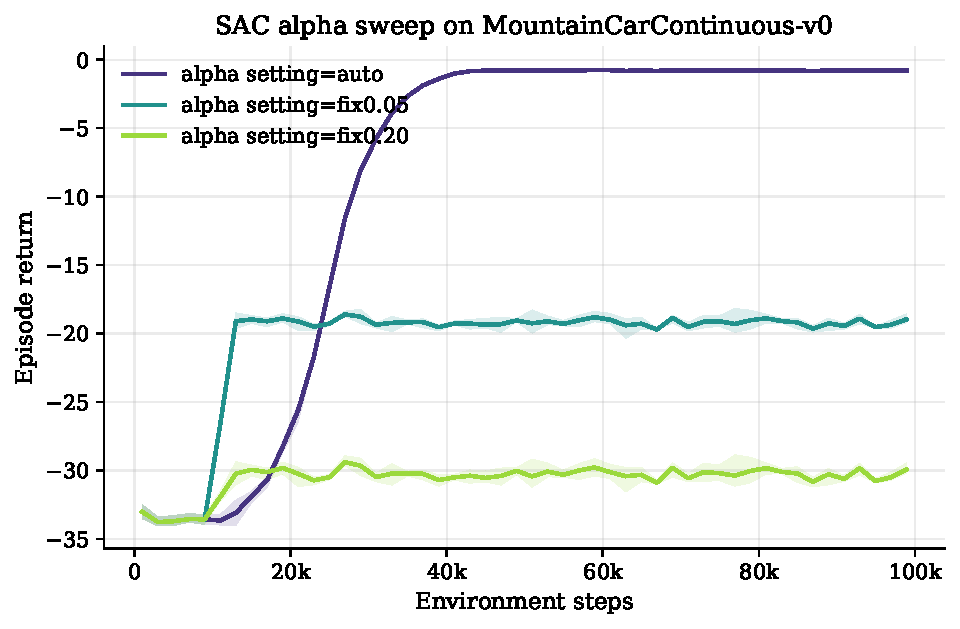
\includegraphics[width=\linewidth]{../plots/ablations/sac_alpha.pdf}\\
            \small \textbf{\algotag[saccol]{SAC} $\alpha$ sweep on MCC.} \\
            Auto, 0.05, 0.20: three failure modes, \hl{0 goals / 9 seeds}.
        \end{minipage}\hfill
        \begin{minipage}[t]{0.46\colwidth}
            \centering
            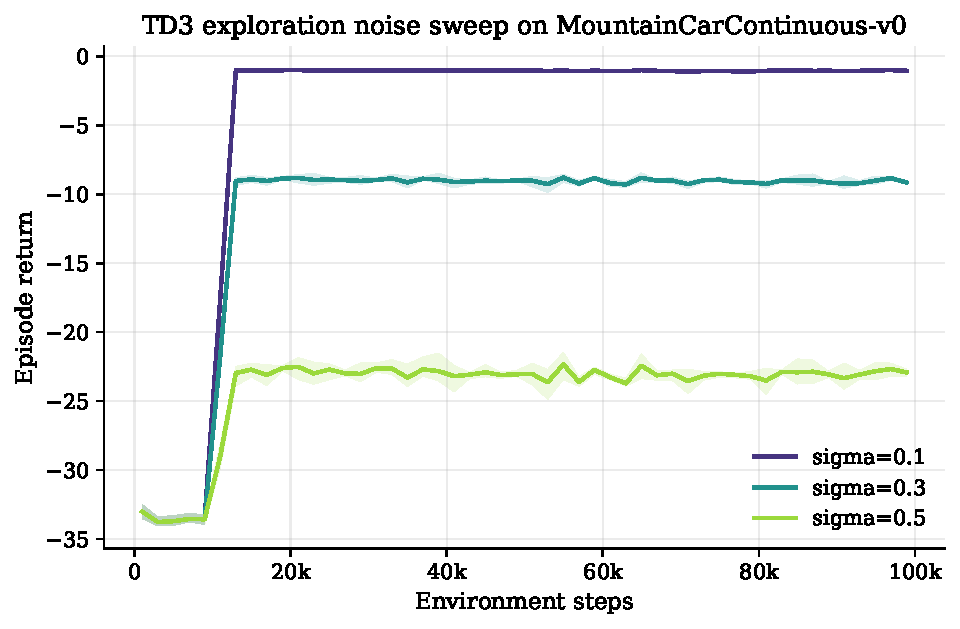
\includegraphics[width=\linewidth]{../plots/ablations/td3_exploration_noise.pdf}\\
            \small \textbf{\algotag[td3col]{TD3} $\sigma$ sweep on MCC.} \\
            $\sigma\in\{0.1, 0.3, 0.5\}$: \hl{more noise is worse}.
        \end{minipage}

        \vspace{0.3em}
        \begin{minipage}[t]{0.46\colwidth}
            \centering
            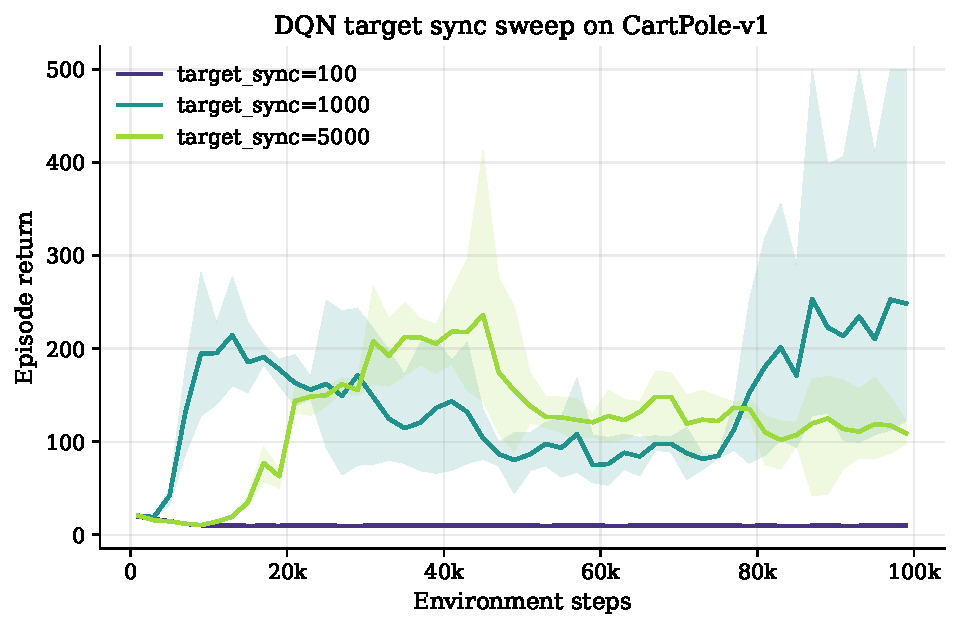
\includegraphics[width=\linewidth]{../plots/ablations/dqn_target_sync.pdf}\\
            \small \textbf{\algotag[dqncol]{DQN} target-sync, CartPole.} \\
            \hl{U-shape}; $\tau{=}1000$ at the edge of stability.
        \end{minipage}\hfill
        \begin{minipage}[t]{0.46\colwidth}
            \centering
            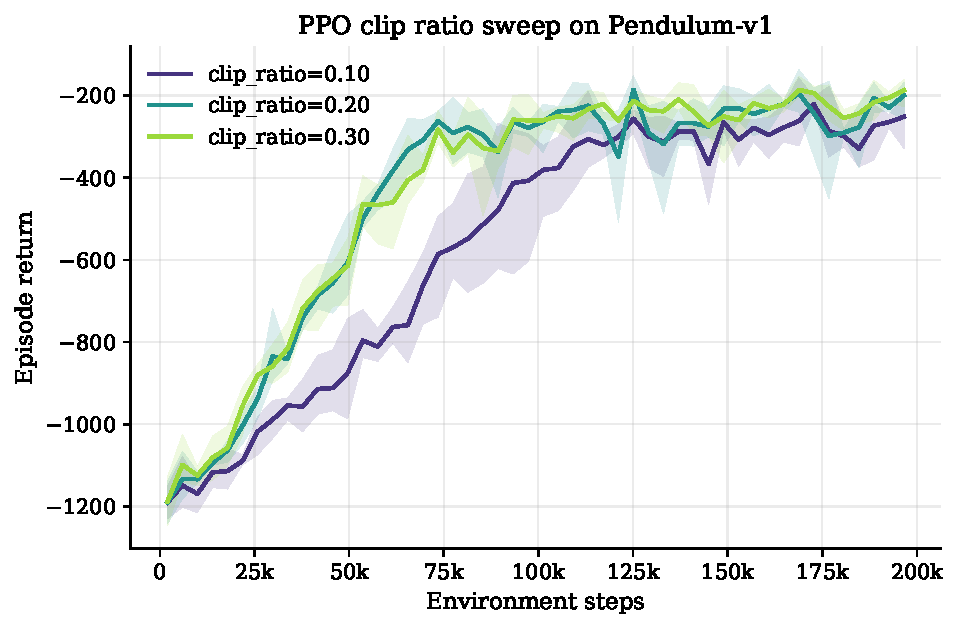
\includegraphics[width=\linewidth]{../plots/ablations/ppo_clip_ratio.pdf}\\
            \small \textbf{\algotag[ppocol]{PPO} clip ratio, Pendulum.} \\
            $\epsilon{=}0.1$ too conservative; 0.2 \& 0.3 tied.
        \end{minipage}

        \vspace{0.25em}
        \small
        \textbf{Why off-policy continuous methods fail on MCC.} Entropy regularization (SAC) and additive Gaussian noise (TD3) drive uniform coverage of the \emph{local} action set, not directed exploration in state space. PPO's on-policy rollouts occasionally produce a long correlated action sequence that crosses the hill; off-policy replay samples are decorrelated and cannot. Structured exploration variants (e.g.\ gSDE) have been shown to close this gap~[6].
    \end{alertblock}

    % ---------- Limitations and open questions ----------
    \begin{block}{6. Limitations \& open questions}
        \begin{itemize}
            \itemsep-0.2em
            \item \textbf{More seeds.} 3 per (algo, env); more would tighten CIs at super-linear cost. Bootstrap CIs are wide enough to keep claims honest.
            \item \textbf{Network width sweep.} Widths fixed at canonical defaults: $(64,64)$ for DQN/PPO, $(256,256)$ for SAC/TD3. The actor-parameter gap is a width choice, not an algorithmic property.
            \item \textbf{Second sparse benchmark.} Generalizing the MCC headline needs e.g.\ \texttt{Reacher} with a binary reward or a sparsified \texttt{Pendulum}.
            \item \textbf{Directed exploration.} Add gSDE~[6], RND, or NoisyNet on top of SAC/TD3 on MCC to test whether directed exploration closes the gap that local entropy/noise cannot.
        \end{itemize}
    \end{block}

    \vfill

\end{column}

\separatorcolumn

% ============================================================
% RIGHT COLUMN
% ============================================================
\begin{column}{\colwidth}

    % ---------- Key numbers at a glance ----------
    \begin{block}{7. Headline numbers}
        \centering
        \begin{tikzpicture}
            \node at (0,0) {\keynum{epflred}{$13\times$}{SAC sample-efficiency over PPO on Pendulum (steps to $-200$)}};
            \node at (10,0) {\keynum{epflred}{$0/9$}{Goal discoveries by SAC across $\alpha$-sweep seeds on MCC}};
        \end{tikzpicture}
    \end{block}

    % ---------- Learning curves ----------
    \begin{block}{8. Learning curves: one figure per environment}
        \vspace{-0.3em}
        \centering
        \begin{minipage}[t]{0.49\colwidth}
            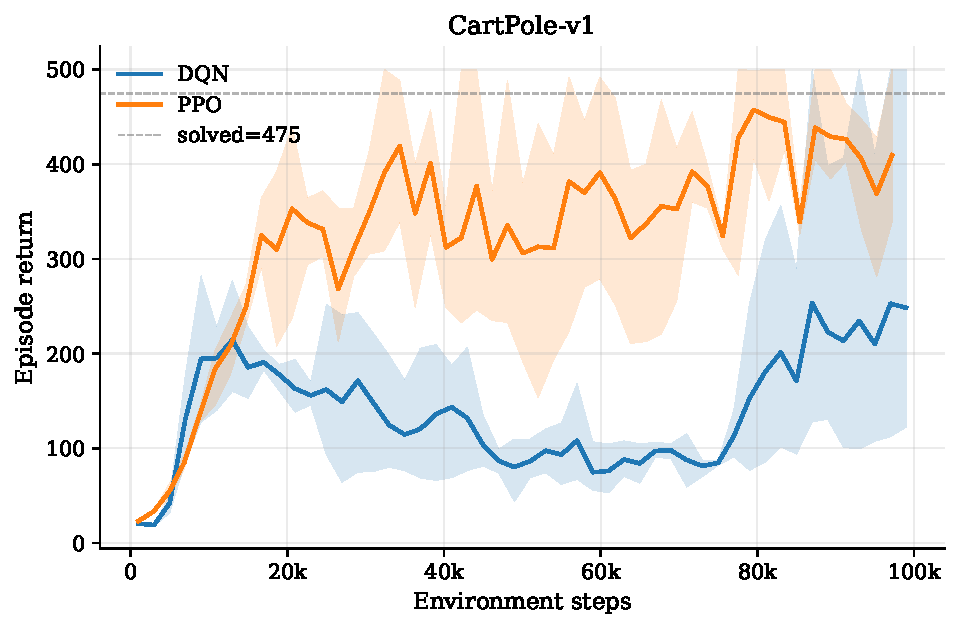
\includegraphics[width=\linewidth]{../plots/per_env/CartPole-v1.pdf}\\
            \small \textbf{CartPole.} \hl{DQN bimodal} (1/3 solve); PPO reliable, 380, CI [350, 402].
        \end{minipage}\hfill
        \begin{minipage}[t]{0.49\colwidth}
            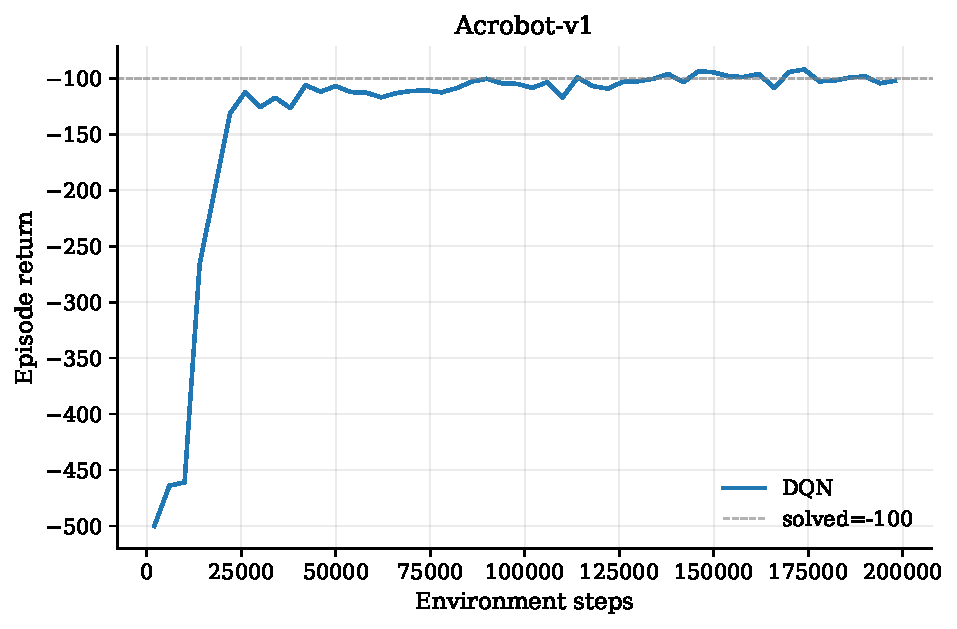
\includegraphics[width=\linewidth]{../plots/per_env/Acrobot-v1.pdf}\\
            \small \textbf{Acrobot.} DQN solves cleanly in $\sim$30k steps; one PPO seed collapses.
        \end{minipage}

        \vspace{0.4em}

        \begin{minipage}[t]{0.49\colwidth}
            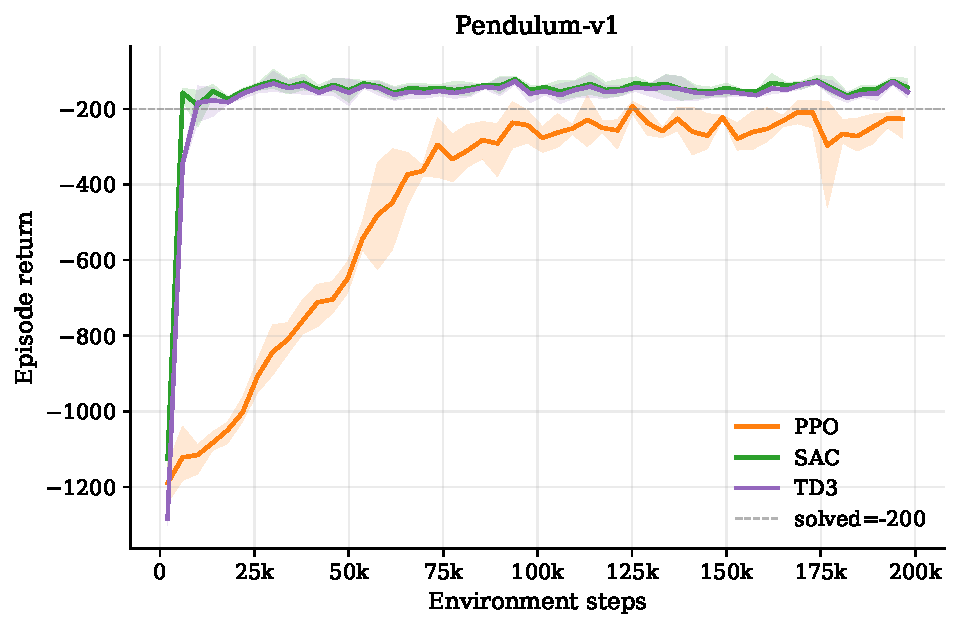
\includegraphics[width=\linewidth]{../plots/per_env/Pendulum-v1.pdf}\\
            \small \textbf{Pendulum.} \hl{SAC and TD3: $\sim 13\times$ more sample-efficient than PPO} (steps to $-200$).
        \end{minipage}\hfill
        \begin{minipage}[t]{0.49\colwidth}
            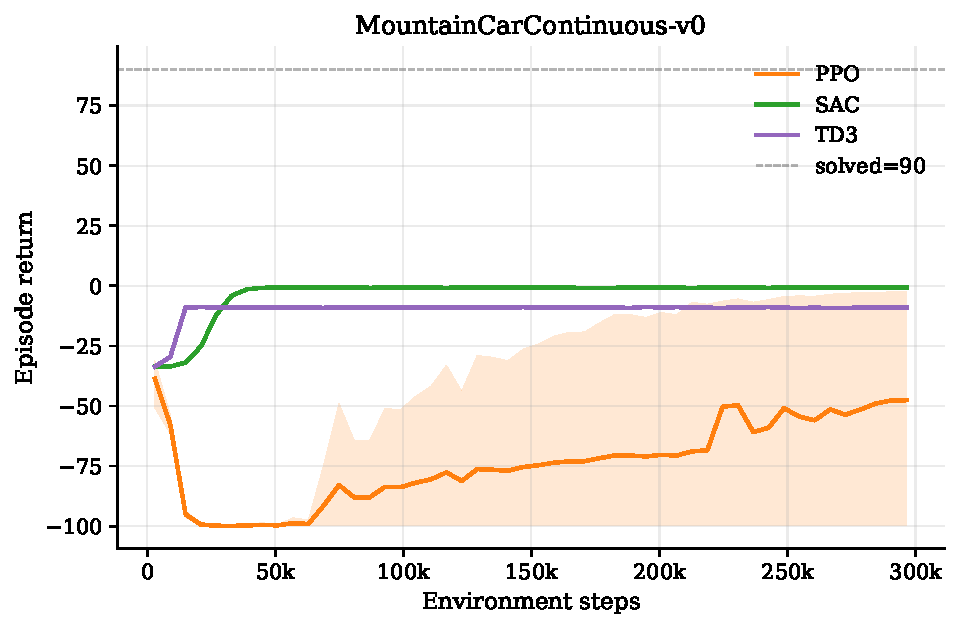
\includegraphics[width=\linewidth]{../plots/per_env/MountainCarContinuous-v0.pdf}\\
            \small \textbf{MCC, sparse.} \hl{Only PPO finds the goal} (\hl{1/3 seeds only}, $-2.5$); SAC and TD3 plateau at a lazy local optimum.
        \end{minipage}
    \end{block}

    % ---------- Bar charts ----------
    \begin{block}{9. Cost, sample efficiency, model size}
        \vspace{-0.3em}
        % Row 1
        \begin{minipage}[t]{0.49\colwidth}
            \centering
            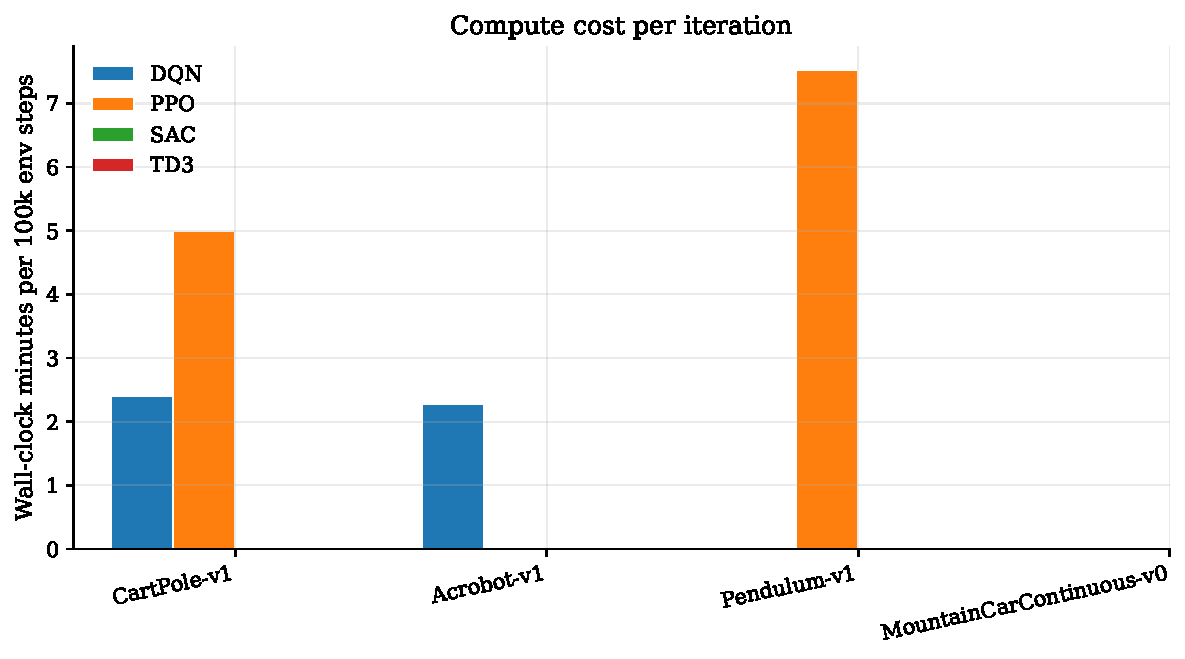
\includegraphics[width=\linewidth]{../plots/bars/wall_clock.pdf}\\
            \small \textbf{Compute}: SAC $>$ TD3 $>$ PPO $>$ DQN.
        \end{minipage}\hfill
        \begin{minipage}[t]{0.49\colwidth}
            \centering
            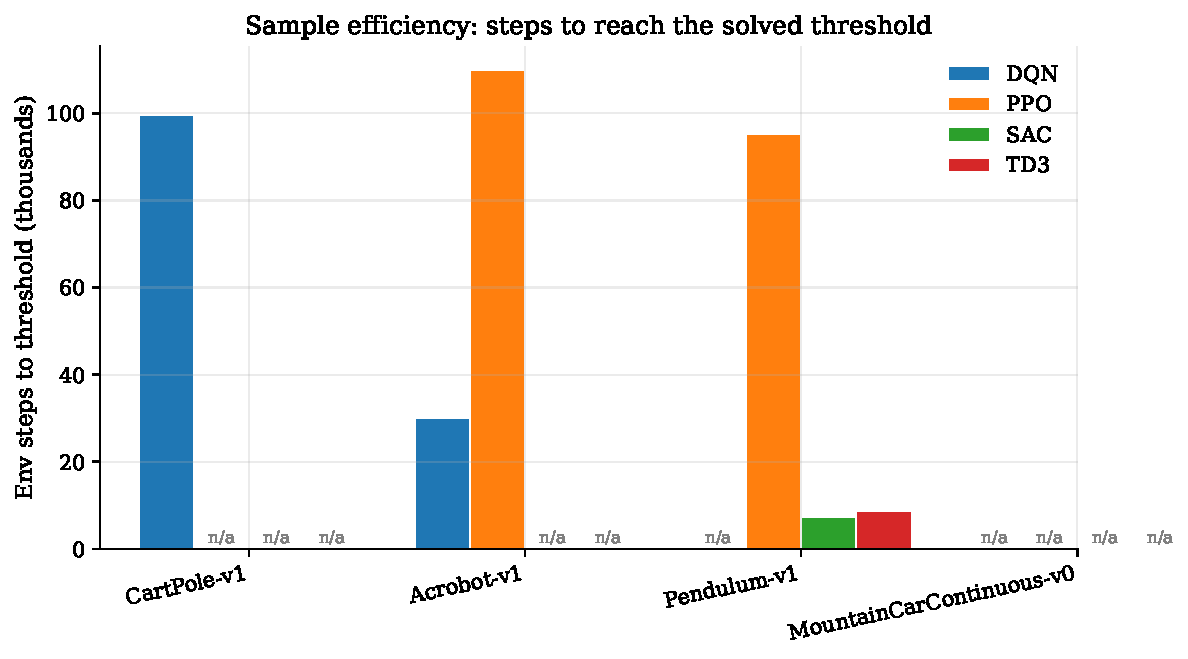
\includegraphics[width=\linewidth]{../plots/bars/sample_efficiency.pdf}\\
            \small \textbf{Sample efficiency} (steps to threshold).
        \end{minipage}

        \vspace{0.4em}
        % Row 2 — centred
        \begin{center}
        \begin{minipage}[t]{0.49\colwidth}
            \centering
            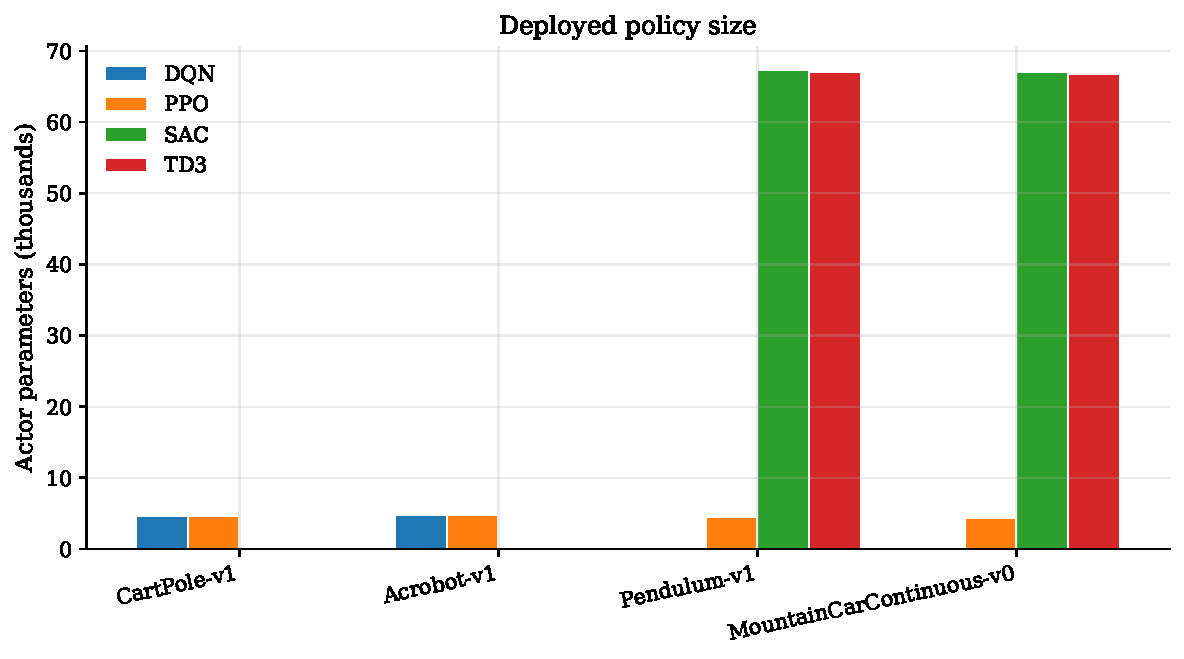
\includegraphics[width=\linewidth]{../plots/bars/param_count.pdf}\\
            \small \textbf{Actor params}, $(64,64)$ vs $(256,256)$.
        \end{minipage}
        \end{center}
    \end{block}

    % ---------- Decision diagram + practical rule ----------
    \begin{exampleblock}{10. When to use which algorithm}
        \centering
        \decisionTree

        \vspace{0.3em}
        \begin{itemize}
            \itemsep0.1em
            \item \textbf{Discrete actions}: \algotag[dqncol]{DQN} fastest on Acrobot ($\sim$30k steps); \algotag[ppocol]{PPO} more reliable on CartPole (avoids bimodality).
            \item \textbf{Dense-reward continuous}: \algotag[saccol]{SAC} and \algotag[td3col]{TD3} dominate, $12.9\times$ over \algotag[ppocol]{PPO} on Pendulum (steps to threshold).
            \item \textbf{Sparse-reward continuous}: \algotag[ppocol]{PPO} is the only one to find the MCC goal (1/3 seeds); the failure of SAC/TD3 is structural in the canonical per-step exploration mechanism, not a tuning issue.
        \end{itemize}
        \centering
        \textbf{\large Pick SAC or TD3 first on continuous control; switch to PPO (or add explicit exploration bonuses) the moment reward becomes sparse.}
    \end{exampleblock}

    % ---------- References + artefacts (combined, compact) ----------
    \begin{block}{References \& project artefacts}
        \small
        \begin{multicols}{2}
        \setlength{\parskip}{0.15em}
        \noindent
        [1] Mnih et al.\ \textit{Playing Atari with Deep RL.} arXiv:1312.5602, 2013.

        \noindent
        [2] Schulman et al.\ \textit{PPO Algorithms.} arXiv:1707.06347, 2017.

        \noindent
        [3] Haarnoja et al.\ \textit{Soft Actor-Critic.} ICML, 2018.

        \noindent
        [4] Fujimoto et al.\ \textit{Addressing Function Approximation Error.} ICML, 2018.

        \noindent
        [5] Towers et al.\ \textit{Gymnasium.} 2023.

        \noindent
        [6] Raffin et al.\ \textit{Smooth Exploration for Robotic RL.} CoRL, 2022.
        \end{multicols}
        \vspace{0em}
        \textbf{Artefacts:} PyTorch from scratch (no \texttt{stable-baselines3});
        per-(algo, env) YAML in \texttt{configs/};
        curves, seed grids, ablations and bar charts under \texttt{plots/};
        bootstrap-CI scoreboard in \texttt{plots/scoreboard.\{csv,tex\}}.
    \end{block}

    \vfill

\end{column}
\separatorcolumn

\end{columns}
\end{frame}
\end{document}